%%%%%%%%%%%%%%%%%%%%%%%%%%%%%%%%%%%%%%%%%%%%%%%%%%%%%%%%%%%%%%%%%%%%%%
% Lớp 10 | Bất phương trình bậc 2 một ẩn | Dấu của tam thức bậc 2
% Dạng 0D7?1-3: Bài toán xét dấu biết BXD, đồ thị
% Số câu: 11  (sinh tự động bởi tach_cau.py; từ nay thầy sửa trực tiếp file này)
%%%%%%%%%%%%%%%%%%%%%%%%%%%%%%%%%%%%%%%%%%%%%%%%%%%%%%%%%%%%%%%%%%%%%%

%%%%%%%%%%%%%%%% TRẮC NGHIỆM 4 PHƯƠNG ÁN %%%%%%%%%%%%%%%%

% nguồn: MaHoaNH_TracNghiem_Lop10
\begin{ex}%[0D7N1-3]%[ma:20ce72c7]
	\immini[thm]{Cho đồ thị hàm số bậc hai $y=f(x)$ tiếp xúc với trục hoành như hình vẽ.  Dấu tam thức bậc hai $f(x)$ đúng với mọi giá trị của $x$ là
	 \choice
		{$f(x)  = 0$}
		 {$f(x)>0$}
		{$f(x) \geq 0$} 
		 {\True $f(x)\leq 0$}}
		 {
		\begin{tikzpicture}[scale=1,font=\footnotesize,line join=round,line cap=round,>=stealth]
				 \draw[->] (-1,0)--(4,0) node[below] {$x$};
				\draw[->] (0,-2.3)--(0,1)  node[left] {$y$};
				 \draw
					(0,0) node  [above right] {$O$} circle (1pt);
				\draw[samples=200,domain=0.5:3.5,smooth,variable=\x] plot  (\x,{(-1)*(\x-2)^2});
			\end{tikzpicture}
		 }
	 \loigiai{
		Ta có đồ thị hàm số bậc  hai $y=f(x)$ nằm phía dưới trục hoành và tiếp xúc với trục hoành nên $f(x)\leq 0$ với mọi $x$.
	 }
\end{ex}

% nguồn: MaHoaNH_TracNghiem_Lop10
\begin{ex}%[0D7N1-3]%[ma:c6cd0727]
	Cho tam thức bậc hai $y=ax^2+bx+c$ với $a\ne  0$ có bảng xét dấu sau
	\begin{center}
		\begin{tikzpicture}
				\tkzTabInit[nocadre=false,lgt=1.2,espcl=2.5,deltacl=0.6] 
					{$x$ /0.6,$f (x)$  /0.6}
					{$-\infty$,$1$,$2$,$+\infty$} 
				\tkzTabLine{,+,$0$,-,$0$,+,} 
			\end{tikzpicture}
	\end{center}
	Dựa vào bảng xét dấu trên cho biết $f(x)\ge  0$ khi $x$ thuộc khoảng nào sau đây?
	 \choice
		 {$(-\infty;+\infty)$}
		 {$(-\infty;2)$}
		{\True  $[2;+\infty)$}
		{$( 1;2)$} 
	\loigiai{ 
		Dựa vào bảng xét dấu, suy ra $f(x)\ge 0\Leftrightarrow x\in \left(-\infty;1\right] \cup  \left[2;+\infty\right)$.
	} 
\end{ex}

% nguồn: MaHoaNH_TracNghiem_Lop10
\begin{ex}%[0D7N1-3]%[ma:2af042bc]
	 \immini{
	Cho hàm số $f(x)=ax^{2}+bx+c$ có đồ thị như hình vẽ. Tìm tất cả giá trị của $x$  để $f(x)<0$.
	\choice 
		{$x\in(-\infty;1)\cup(3;+\infty)$} 
		{\True $x\in(1;3)$} 
		{$x\in(0;2)$} 
		 {$x\in(-1;0)$}
		 }{
		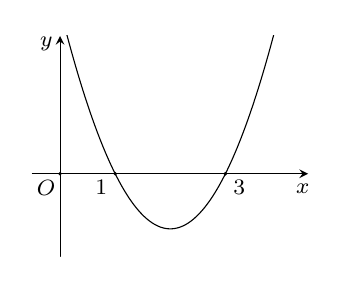
\begin{tikzpicture}[scale=0.7,font=\footnotesize,line join=round,line cap=round,>=stealth]
				\def  \xmin{-.5}
				\def \xmax{4.5} 
				 \def \ymin{-1.5}
				\def  \ymax{2.5}
				\draw[->]  (\xmin,0)--(\xmax,0) node[shift=(-110:0.2)] {$x$};
				\draw[->] (0,\ymin)--(0,\ymax) node[shift=(-150:0.2)]  {$y$};
				 \fill (0,0) circle (1pt) node[shift=(-135:0.25)]{$O$}
					 (1,0) circle (1pt) node[shift=(-135:0.25)]{$1$}
					(3,0) circle  (1pt) node[shift=(-45:0.25)]{$3$};
				 \clip (\xmin,\ymin) rectangle (\xmax,\ymax);
				\draw[smooth,samples=100,domain=\xmin:\xmax]  plot (\x,{(\x)^2-4*(\x)+3});
			\end{tikzpicture}
		} 
	 \loigiai{
		Vì $f(x)<0$  nên ta tìm các giá trị $x$ ứng với phần đồ thị nằm phía dưới trục hoành.\\
		Vậy $x\in(1;3)$. 
	} 
\end{ex}

% nguồn: MaHoaNH_TracNghiem_Lop10
\begin{ex}%[0D7H1-3]%[ma:de819fe9]
	Biểu  thức nào sau đây có kết quả xét dấu cho bởi bảng:
	\begin{center}
		\begin{tikzpicture}
				\tkzTabInit[nocadre=false,lgt=1.2,espcl=3.5,deltacl=0.6] 
					{$x$/0.8,$f (x)$/1} 
					 {$-\infty$,$0$,$3$,$+\infty$}
				 \tkzTabLine{,+,z,-,z,+,}
			\end{tikzpicture}
	\end{center}
	 \choice
		 {$f(x)=\dfrac{x}{x+3}$}
		 {$f(x)=\dfrac{x-3}{x}$}
		{\True $f(x)=x(x-3)$} 
		 {$f(x)=x(3-x)$}
	\loigiai{Đây là bảng xét dấu của hàm số bậc hai có giao điểm với trục hoành tại điểm có hoành độ $x=0$ và $x=3$ có hệ số  $a>0$.\\
	Vậy biểu thức có kết quả xét dấu như trên  là $f(x)=x(x-3)$.}
\end{ex}

% nguồn: MaHoaNH_TracNghiem_Lop10
\begin{ex}%[0D7H1-3]%[ma:299a992c]
	Bảng xét dấu sau  của tam thức bậc hai nào?
	\begin{center}
		\begin{tikzpicture}[>=stealth]
				\tkzTabInit[nocadre=false,lgt=1.5,espcl=2,deltacl=0.6]{$x$/.7,$f  (x)$/.7}
					 {$-\infty$,$-3$,$2$,$+\infty$}
				 \tkzTabLine{,-,$0$,+,$0$,-,}
			\end{tikzpicture}
	\end{center}
	 \choice
		{$f(x)=x^2-x-6$} 
		{\True $f(x)=-x^2-x+6$} 
		 {$f(x)=-x^2+x+6$}
		 {$f(x)=x^2+x-6$}
	 \loigiai{
		Từ bảng xét dấu ta thấy hệ số  của $x^2$ âm
		và $f(x)=0$ có 2 nghiệm $x=-3$,  $x=2$.
	 }
\end{ex}

% nguồn: MaHoaNH_TracNghiem_Lop10
\begin{ex}%[0D7H1-3]%[ma:c6a9c297]
	Bảng xét dấu sau là của tam thức bậc hai  nào?
	\begin{center}
		\begin{tikzpicture}[>=stealth]
				\tkzTabInit[nocadre=false,lgt=1.5,espcl=2,deltacl=0.6]{$x$/.7,$f (x)$/.7} 
					{$-\infty$,$1$,$2$,$+\infty$} 
				 \tkzTabLine{,-,$0$,+,$0$,-,}
			\end{tikzpicture}
	\end{center}
	\choice 
		{$f(x)=-x^2-3x+2$} 
		{\True $f(x)=\left(x-1\right)\left(-x+2\right)$} 
		 {$f(x)=x^2+3x+2$}
		 {$f(x)=x^2-3x+2$}
	\loigiai{ 
		Dựa vào bảng xét  dấu, ta có
		\begin{itemize}
			\item $f(x)$  có nghiệm là $1$ và $2$ nên loại $f(x)=-x^2-3x+2$ và $f(x)=x^2+3x+2$;
			\item $\forall x\in \left(1;  2\right),f(x) > 0$ nên $a < 0$. Do đó đáp án $f(x)=x^2-3x+2$ sai;
			\item Đáp án  $f(x)=\left(x-1\right)\left(-x+2\right)$ đúng.
		\end{itemize}
	} 
\end{ex}

% nguồn: MaHoaNH_TracNghiem_Lop10
\begin{ex}%[0D7H1-3]%[ma:2858d794]
	Bảng xét  dấu sau là của biểu thức nào?
	\begin{center}
		\begin{tikzpicture}[>=stealth]
				\tkzTabInit[nocadre=false,lgt=1.5,espcl=2,deltacl=0.6]{$x$/.7,$f (x)$/.7} 
					{$-\infty$,$-2$,$-1$,$+\infty$} 
				 \tkzTabLine{,-,$0$,+,$0$,-,}
			\end{tikzpicture}
	\end{center}
	\choice 
		{$f(x)=(x-1)(x+2)$} 
		 {$f(x)=(x+1)(x+2)$}
		 {$f(x)=x^2-3x+2$}
		 {\True $f(x)=-x^2-3x-2$}
	\loigiai{ 
		 Dựa vào bảng xét dấu, ta thấy
		\begin{itemize}
			 \item $f(x)=0$ có hai nghiệm $x=-1$ và $x=-2$.
			\item  $a<0$.
		\end{itemize}
		Do đó bảng  xét dấu trên là của tam thức $f(x)=-x^2-3x-2$.
	} 
\end{ex}

% nguồn: MaHoaNH_TracNghiem_Lop10
\begin{ex}%[0D7H1-3]%[ma:cd3d01e9]
	Cho $f(x)=ax^2+b x+c\, \left(a\ne 0\right)$ có bảng  xét dấu dưới đây
	\begin{center}
		\begin{tikzpicture}[>=stealth]
				\tkzTabInit[nocadre=false,lgt=1.5,espcl=2,deltacl=0.6]{$x$/.7,$f  (x)$/.7}
					{$-\infty$,$x_1$,$x_2$,$+\infty$} 
				\tkzTabLine{,+,$0$,-,$0$,+,} 
				\path ($(L1)!.5!(L2)$) node{$0$}; 
			\end{tikzpicture}
	\end{center}
	Hỏi mệnh  đề nào dưới đây đúng?
	\choice 
		{\True $a  > 0,b < 0,c > 0$}
		{$a < 0,b < 0,c  > 0$}
		{$a > 0,b  > 0,c > 0$}
		 {$a > 0,b < 0,c < 0$}
	 \loigiai{
		\begin{itemize}
			\item Tại $x=0$ thì $f(0)=c >  0$.
			\item Trong khoảng hai nghiệm $\left(x_1;x_2 \right)$, $f(x)$ mang dấu  \lq\lq$-$\rq\rq\, nên $a > 0$.
			\item Phương trình $f(x)=0$ có hai nghiệm $x_1, x_2$ thỏa mãn $0< x_1 < x_2$ $\Rightarrow x_1+x_2 >  0$.
			\item Theo định lý Vi-ét $x_1+x_2=\dfrac{-b}{a}$ nên  $\dfrac{-b}{a} > 0\Rightarrow b < 0$.
		\end{itemize}
	 }
\end{ex}


%%%%%%%%%%%%%%%% ĐÚNG/SAI %%%%%%%%%%%%%%%%

% nguồn: MaHoaNH_DungSai_Lop10
\begin{ex}%[0D7H1-3]%[ma:c636923d]
	\immini[thm]{ 
	 Cho hàm số bậc hai $f(x)=x^2+x+1$ có đồ thị như hình bên.
	\choiceTF 
		{Tam thức bậc hai $f(x)$  có một nghiệm là $x=1$}
		{\True Tam thức  bậc hai $f(x)$ vô nghiệm}
		{\True Tam thức bậc hai $f(x)$ dương với mọi $x\in\mathbb{R}$} 
		{Tam thức bậc hai $f(x)$  dương với mọi $x\neq 1$}
		}{ 
		\begin{tikzpicture}[scale=0.6,font=\footnotesize,line join=round,line cap=round,>=stealth]
				 \tikzset{label style/.style={font=\footnotesize}}
				\def \xmin{-4} \def \xmax{3} 
				\def  \ymin{-1.5} \def \ymax{5.5}
				\def\a{1} \def\b{1}  \def\c{1}
				\draw[->]  (\xmin,0) -- (\xmax,0) node[below]{$x$};
				\draw[->] (0,\ymin)  -- (0,\ymax) node[right]{$y$};
				\tkzDefPoints{0/0/O,0/1/A} 
				 \tkzDrawPoints[fill=black](O,A)
				\foreach  \x/\g in {O/-135}
				\draw  (\x) node[shift={(\g:.3)}]{$\x$};
				\begin{scope}
					\clip (\xmin,\ymin) rectangle  (\xmax,\ymax);
					 \draw[thick,color=black,smooth,samples=100,domain=\xmin:\xmax] plot (\x,{\a*(\x)^2 +\b*(\x)+\c});
				\end{scope}
				\foreach  \p/\g in {1/0} \draw (0,\p) node[shift={(\g:.225)}]{$\p$}--+(.05,0)--+(-.05,0);
			\end{tikzpicture}
		} 
	 \loigiai{
		Từ đồ thị, ta thấy tam thức bậc hai $f(x)=x^2+x+1$  dương với mọi $x\in\mathbb{R}$.
	 }
\end{ex}

% nguồn: MaHoaNH_DungSai_Lop10
\begin{ex}%[0D7H1-3]%[ma:f8667a61]
	 \immini[thm]{
	Cho hàm số bậc hai $f(x)=x^2+1{,}5x-1$  có đồ thị như hình bên.
	\choiceTF 
		{\True Tam thức  bậc hai $f(x)$ có hai nghiệm phân biệt}
		{\True Tam thức bậc hai $f(x)$ âm trong khoảng  $\left(-2;\dfrac{1}{2}\right)$}
		{Tam thức bậc hai $f(x)$  dương tại $x=\dfrac{1}{3}$}
		 {Tam thức bậc hai $f(x)$ âm tại $x=-3$}
		 }{
		\begin{tikzpicture}[scale=0.6,font=\footnotesize,line join=round,line cap=round,>=stealth]
				 \tikzset{label style/.style={font=\footnotesize}}
				\def \xmin{-4} \def \xmax{3} 
				\def \ymin{-3} \def  \ymax{4}
				\def\a{1} \def\b{1.5} \def\c{-1} 
				\draw[->] (\xmin,0) -- (\xmax,0) node[below]{$x$}; 
				\draw[->]  (0,\ymin) -- (0,\ymax) node[right]{$y$};
				\tkzDefPoints{0/0/O,-2/0/A,0.5/0/B} 
				 \tkzDrawPoints[fill=black](O,A,B)
				\foreach  \x/\g in {O/-135}
				\draw (\x)  node[shift={(\g:.3)}]{$\x$};
				\begin{scope}
					\clip (\xmin,\ymin) rectangle  (\xmax,\ymax);
					\draw[thick,color=black,smooth,samples=100,domain=\xmin:\xmax] plot (\x,{\a*(\x)^2 +\b*(\x)+\c}); 
				\end{scope}
				\foreach \p/\g  in {-2/-90} \draw (\p,0) node[shift={(\g:.25)},xshift=-4pt]{$\p\phantom{-}$}--+(0,.05)--+(0,-.05);
				\foreach \p/\g  in {0.5/-90} \draw (\p,0) node[shift={(\g:.4)}]{$\frac{1}{2}$}--+(0,.05)--+(0,-.05);
			\end{tikzpicture}
		 }
	 \loigiai{
		Từ đồ thị, ta  thấy tam thức bậc hai $f(x)=x^2+x+1$ dương trong các khoảng $\left(-\infty;-2\right)$, $\left(\dfrac{1}{2};+\infty\right)$ và âm trong khoảng $\left(-2;\dfrac{1}{2}\right)$.
	} 
\end{ex}


%%%%%%%%%%%%%%%% TRẢ LỜI NGẮN %%%%%%%%%%%%%%%%

% nguồn: MaHoaNH_TraLoiNgan_Lop10
\begin{bt}%[0D7H1-3]%[ma:bbfd096e]
	Cho tam thức  bậc hai $f(x) = x^2 - (2m+3)x + m^2 + 3m$, $m$ là tham số. Có bao nhiêu giá trị nguyên của tham số $m$ để $f(x) < 0, \forall x \in (-1;0)$.
	\shortans{3} 
	 \loigiai{
		Ta có $f(x) = 0 \Leftrightarrow \hoac{&x = m  \\& x = m+3}$\\
		$f(x) < 0 \Leftrightarrow x \in (m; m+3)$\\ 
		Do đó $f(x) < 0, \forall x  \in (-1;0)$
		\begin{eqnarray*}
			&\Leftrightarrow& (-1;0)  \subset (m; m+3)\\
			&\Leftrightarrow& \begin{cases} m \le -1 \\ 0 \le m+3
		\end{cases}\\
		&\Leftrightarrow& \begin{cases} m \le -1 \\ -3 \le m
	\end{cases}\\
	&\Leftrightarrow& -3 \le  m \le -1.
	\end{eqnarray*}
	Vì $m\in\mathbb{Z}$ nên $m \in \{-3;-2;-1\}$, vậy có 3 giá  trị nguyên thỏa mãn.
 }
\end{bt}
